% !TeX root = ../../thesis.tex
\chapter{Results}\label{ch:results}

\section{Hepatitis B phylogeography}

\subsection{Demographic reconstruction}

For this project, we had originally planned to reconstruct the demographic history of Hepatitis B genotypes throughout their history using a Bayesian skygrid coalescent model.
This was a process by which we divided the evolutionary history of the virus into discrete intervals, then attempted to treat each ``bin'' as a constant population size time window---resulting in a population function over time that was piecewise constant.
Bins would then be smoothed with their neighbors to make a continuous estimation of population size through time.

Unfortunately, this process was unsuccessful.
The initial cause of the lack of success was the so-called ``block'' operator of the \gls{mcmc} that governed the change in Skygrid population size values.
This operator became ``stuck'' in all cases where we attempted to use it, such that the \gls{mcmc} algorithm would never accept new proposals in state space, and therefore the simulated parameter values never changed---that is to say, the entire Markov chain became stuck in a local optimum and was never able to leave it.
We attempted to rectify this situation by changing to a different transition kernel---a Hamiltonian Monte Carlo operator---however this operator was still never able to explore the state space rapidly enough to produce results.

To circumvent these issues, we transitioned to using a less sophisticated demographic model wherein the entire population size was assumed to be constant throughout history.
Using this method, we recovered that \gls{hbv}-A had an inferred effective population size of 1,620 [95\% HPD:765--2,815] and that \gls{hbv}-D had an inferred effective population size of 60,686 [95\% HPD: 38,478--86,598].

\subsection{Temporal signal and clock rates}

\newglossaryentry{tmrca}{name={tMRCA},description={Time to most recent common ancestor}}
The mean evolutionary rate and times to the most recent common ancestor (\gls{tmrca}) were first estimated for all datasets without including any ancient sequences (and hence not imposed any informative prior information) by collaborators.
\gls{hbv} genotype A was estimated to evolve at a mean rate of $5.75\times10^{-4}$ [95\% HPD: $3.81\times10^{-4}$--$7.90\times10^{-4}$] substitutions/site/year, genotype D at a mean rate of $1.27\times10^{-3}$ [95\% HPD: $1.12\times10^{-3}$--$1.43\times10^{-3}$] substitutions/site/year, and genotype E at a mean rate of $6.84\times10^{-4}$ [95\% HPD: $2.08\times10^{-4}$--$1.16\times10^{-3}$] substitutions/site/year.
However, \gls{hbv} often shows very little temporal signal, making it difficult to accurately estimate the time scale for an \gls{hbv} phylogeny and to hence put accurate dates on historical migrations of the virus.
M{\"u}hlemann et al. (2018) have shown that including ancient genomic sequences can provide the required additional information to warrant the use of molecular clock models to reconstruct time-measured phylogenetic trees for \gls{hbv}.
For \gls{hbv} datasets A and D, we have hence included the relevant ancient sequences and have set an informative prior distribution on the mean of the underlying lognormal distribution for the uncorrelated relaxed clock model, based on the reported estimate from M{\"u}hlemann et al. (2018).
For genotype A, this leads us to obtain a somewhat increased mean rate of $7.32\times10^{-4}$ [95\% HPD: $4.14\times10^{-4}$--$1.06\times10^{-3}$] substitutions/site/year, while for genotype D we obtained a much decreased mean rate of $9.65\times10^{-5}$ [95\% HPD: $5.97\times10^{-5}$--$1.36\times10^{-4}$] substitutions/site/year.

\subsection{Phylogenetic placement}

An initial goal of ours was to phylogenetically place the 118 complete genome sequences (split among \gls{hbv} genotypes A,D, and E) which were provided to us by collaborators into discrete subgenotype-level categories.
This was done by performing phylogenetic inference on the full set of genomes, then located the new sequences within the context of preexisting genetic diversity for their respective genotypes.
Using this method, we were able to infer putative subgenotypes for each new sequence.
For the genotypes that we analyzed, 54 belong to \gls{hbv} genotypes A and D---the only genotypes we consider for which subgenotype definitions exist.
The remaining 64 new sequences that we introduce come from \gls{hbv}-E; we find that these novel genomes span the existing known diversity of the genotype (Fig.~\ref{fig:HBV-E_new_sequences}).

The most frequent \gls{hbv}-A subgenotypes (Fig.~\ref{fig:HBV-A_new_sequences}) identified were A1 (n = 27, 57.4\%), quasi-subgenotype A3 (n = 11, 23.4\%) including previous [ A3(n = 5, 10.6\%), A4 (n = 4, 8.6\%) and A5 (n = 2, 4.3\%)], and A6 (n = 4, 8.6\%).
Interestingly, phylogenies revealed that two African isolates (ID: MB-135 and MB-146) belonging to \gls{hbv} genotype A did not cluster with any of the known subgenotypes.
Our analysis also reveals that some \gls{hbv}-A sequences with a previously identified subgenotype do not cluster phylogenetically with other members of their subgenotype.
These inconsistencies manifest as three sequences identified as A1, falling independently within the A2 subgenotype.
We also find a single sequence A2 sequence that clusters phylogenetically within A1.

Interestingly, a similar lineage was observed in the phylogenetic tree of genotype D strains of this study.
While 6 out of 8 \gls{hbv} genotype D isolates (Fig.~\ref{fig:HBV-D_new_sequences}) were phylogenetically classified as subgenotypes D1 (n = 4, 57.1\%), D2 (n = 2, 28.6\%) and D7 (n = 1, 14.3\%), two strains (ID: MB-46 and MB-96) did not cluster with any of the \gls{hbv} subgenotype D1-D9 references sequences.


\begin{figure}[ht]
  \centering
  \medskip
  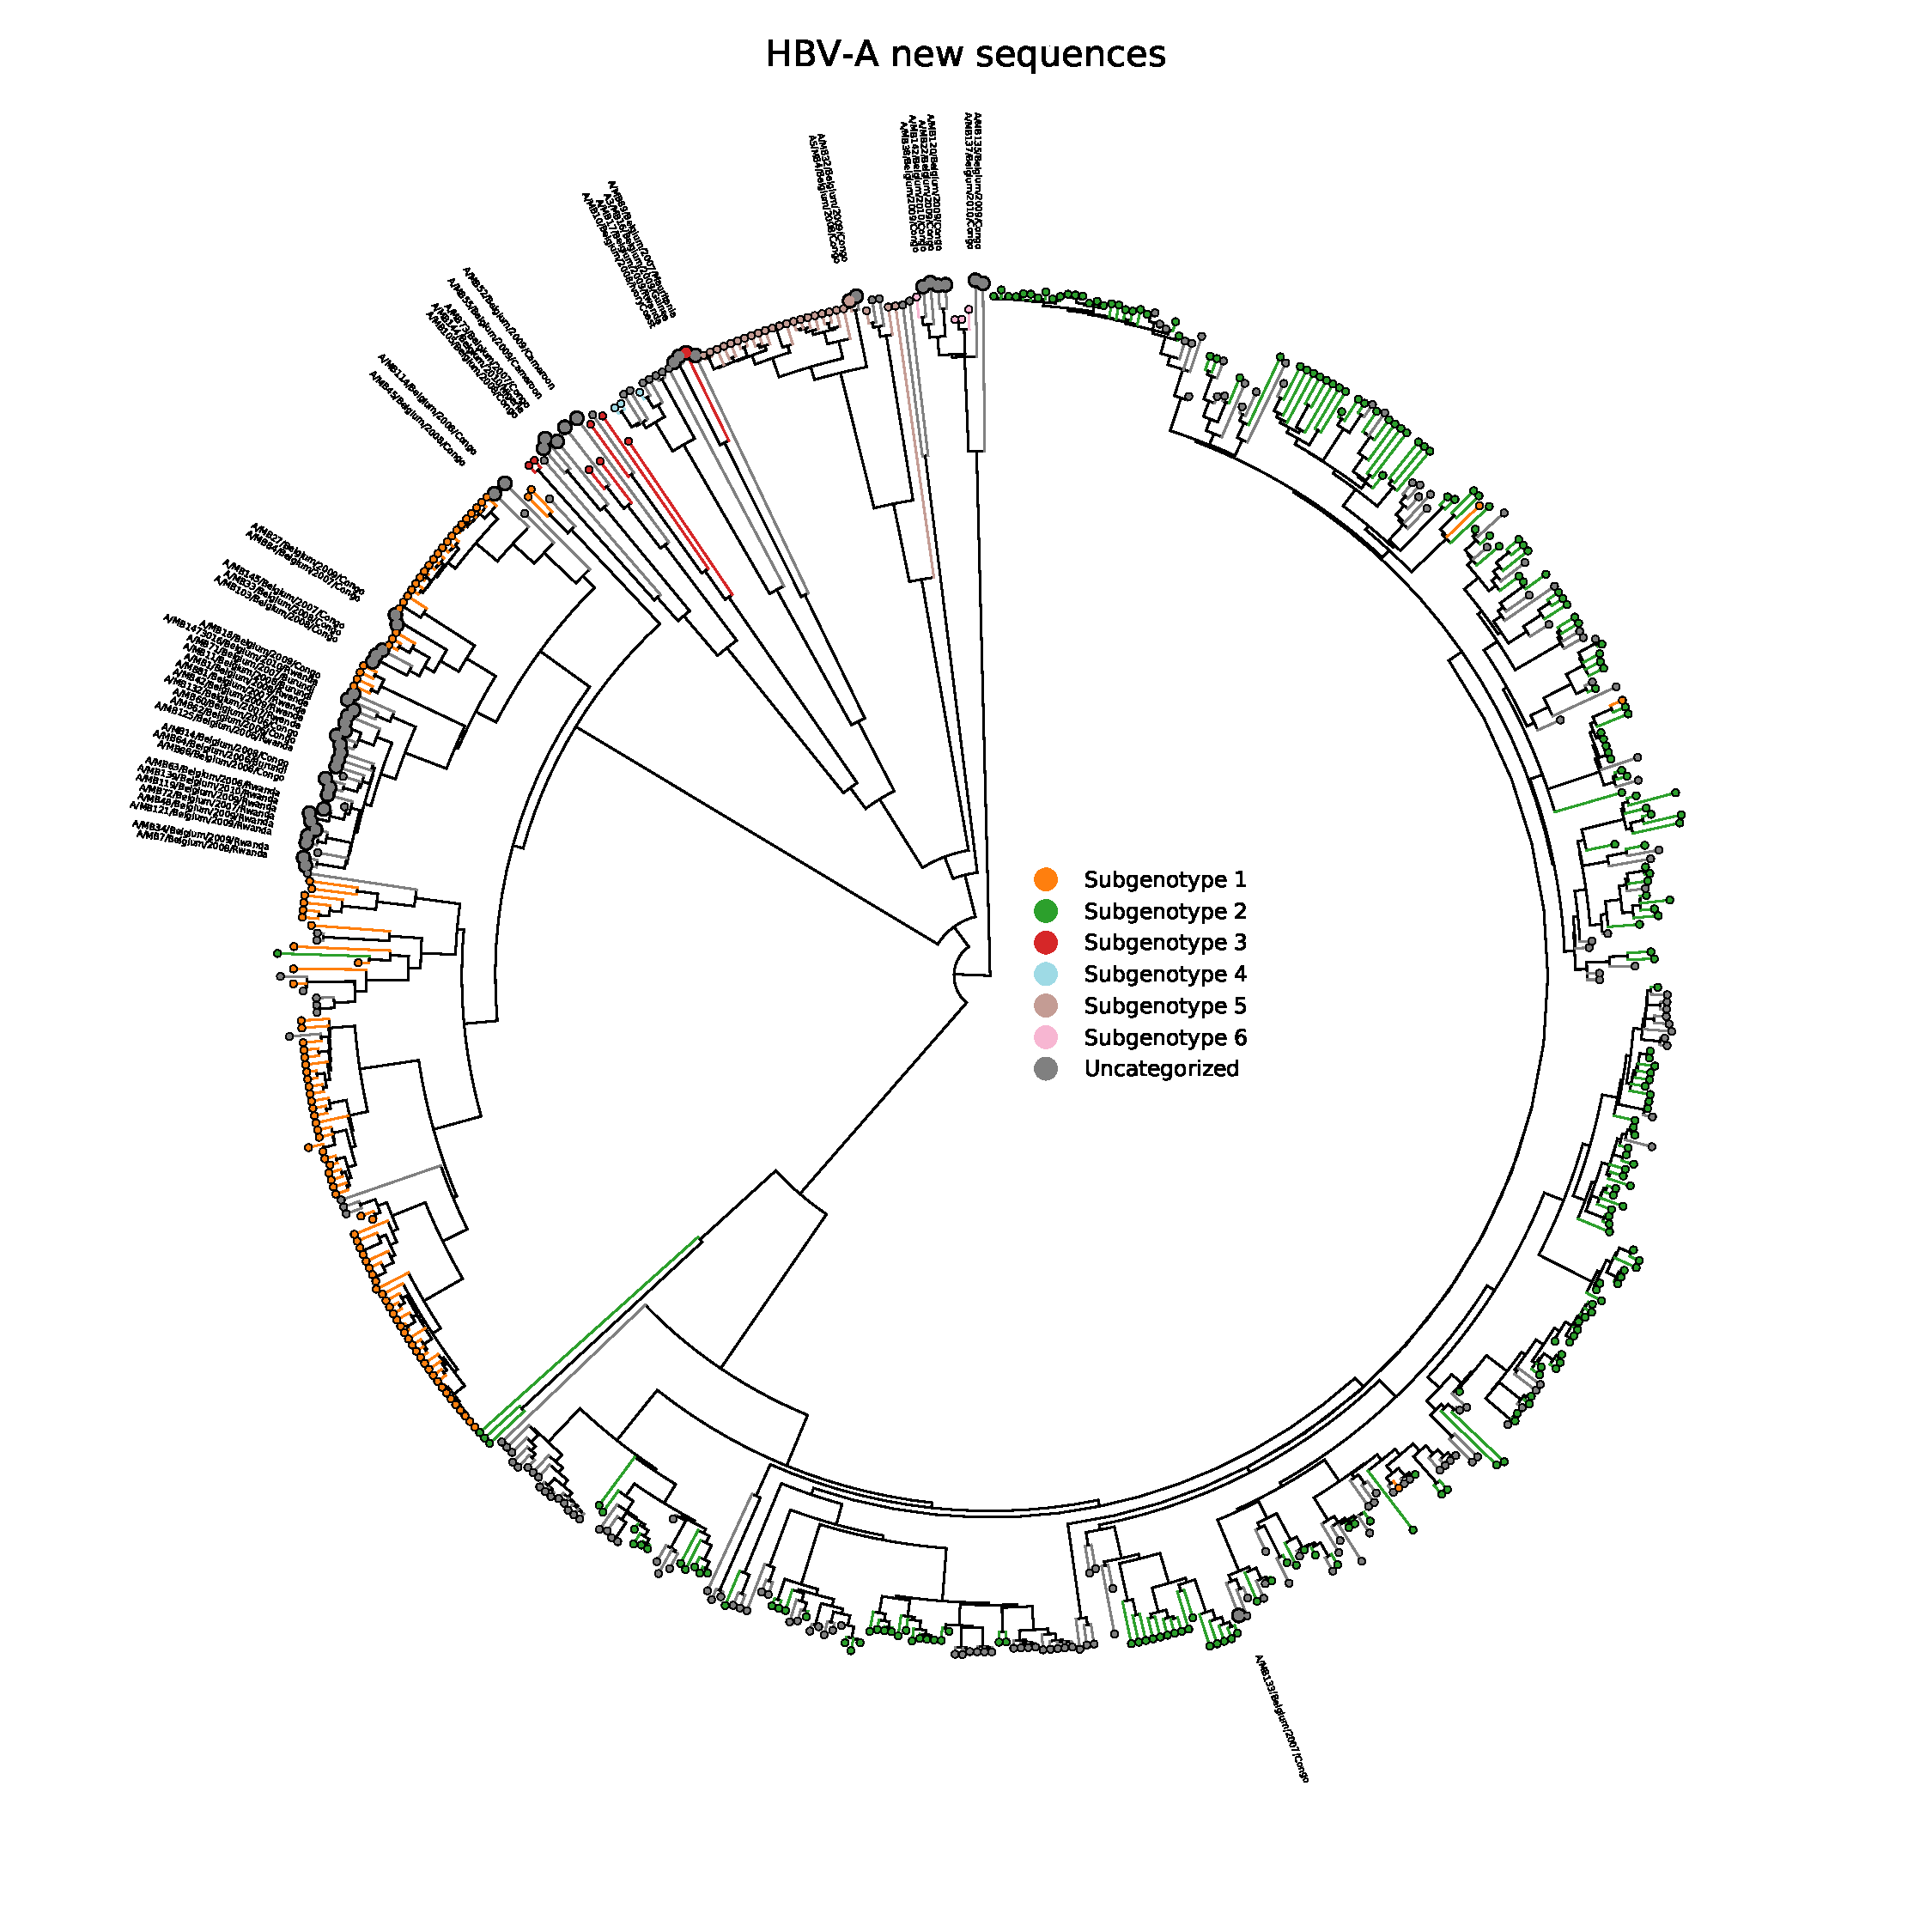
\includegraphics[width=\textwidth]{HBV-A_new_sequences}
  \caption[HBV-A New sequences]{Phylogenetic trees (ancient sequences removed, ancient branch lengths rescaled for visibility) representing the diversity of the novel sequences from this study. Our sequences are shown as enlarged, labeled tips on the phylogeny. Taxa with a known subgenotype are colored by their subgenotype. Out of a total of 47 new genomes, we introduce 29 genomes that cluster most closely with Subgenotype 1, 22 of which represent a closely related subclade. Additionally, we introduce one genome that appears to fall within Subtype 2, nine new genomes that lie within the diversity of Subgenotype 3, two genomes that cluster with Subgenotype 5, and six genomes that cluster most closely with Subgenotype 6.}
  \label{fig:HBV-A_new_sequences}
\end{figure}

\begin{figure}[ht]
  \centering
  \medskip
  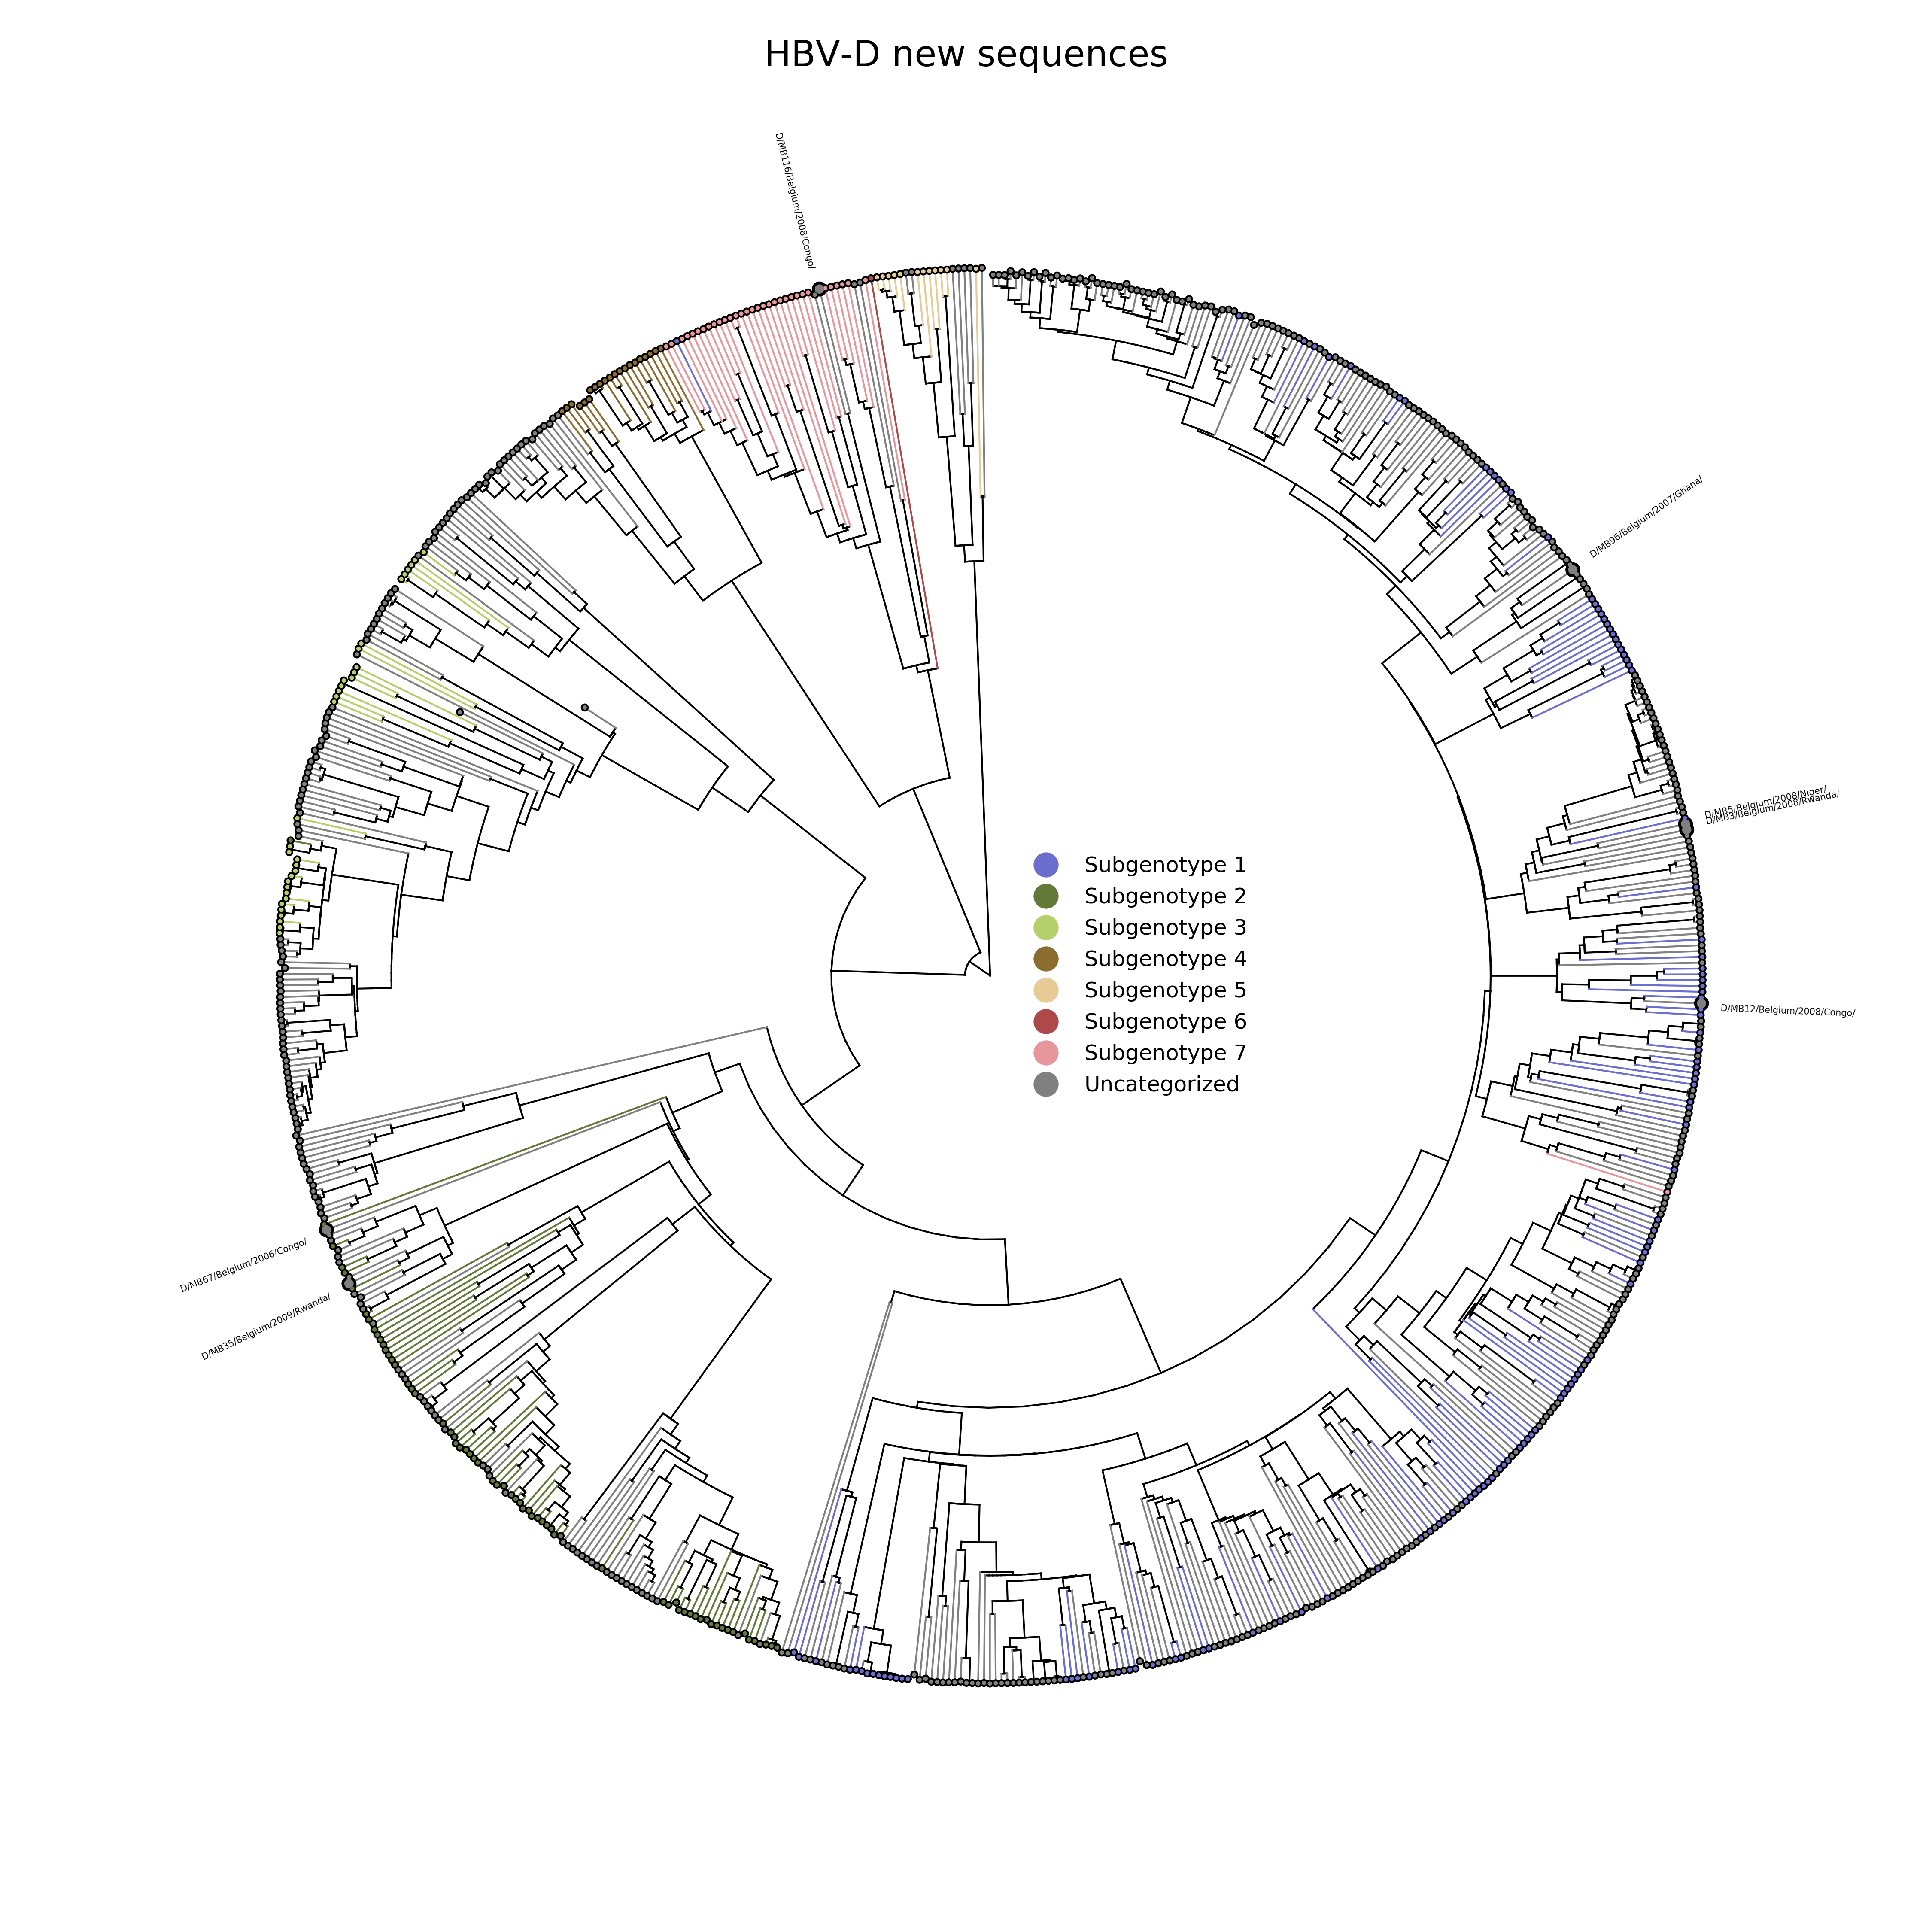
\includegraphics[width=\textwidth]{HBV-D_new_sequences}
  \caption[HBV-D New sequences]{Phylogenetic trees (ancient sequences removed, ancient branch lengths rescaled for visibility) representing the diversity of the novel sequences from this study. Our sequences are shown as enlarged, labeled tips on the phylogeny. Taxa with a known subgenotype are colored by their subgenotype. Here we introduce four novel genomes that fall within the known diversity of Subgenotype 1, two genomes that fall within Subgenotype 2, and one genome in Subgenotype 7.}
  \label{fig:HBV-D_new_sequences}
\end{figure}

\begin{figure}[ht]
  \centering
  \medskip
  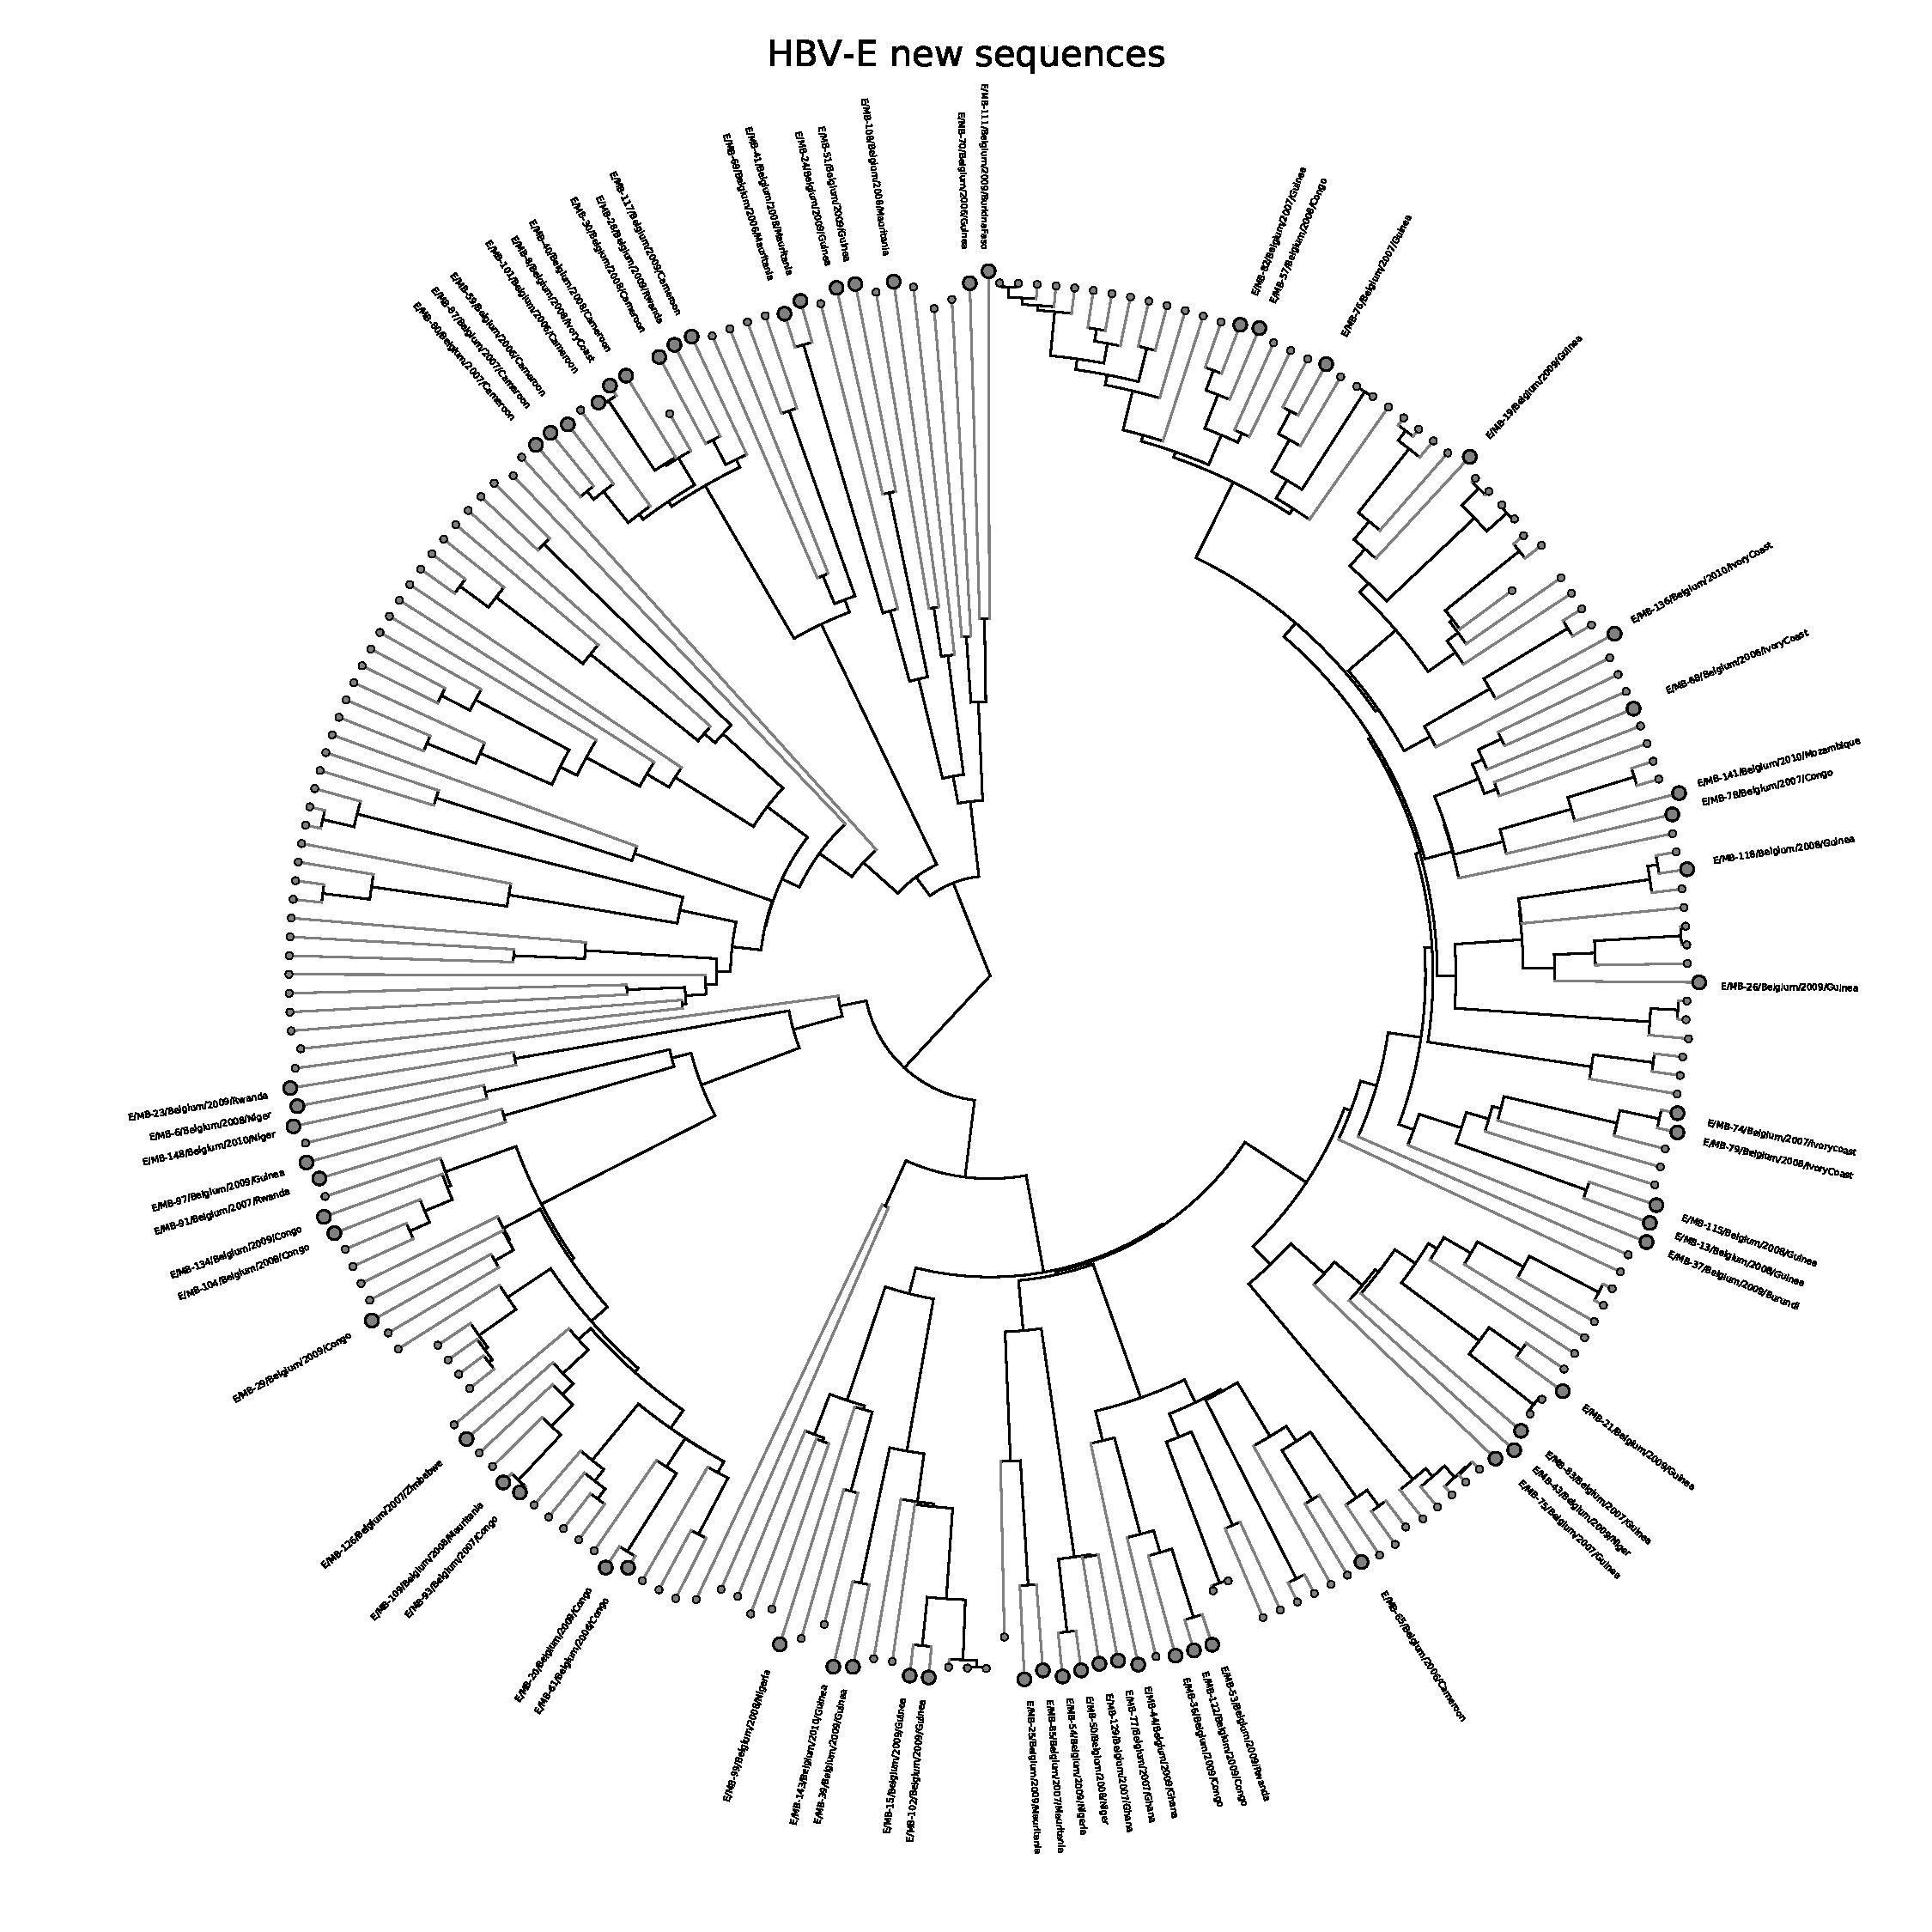
\includegraphics[width=\textwidth]{HBV-E_new_sequences}
  \caption[HBV-E New sequences]{Phylogenetic trees representing the diversity of the novel sequences from this study. Our sequences are shown as enlarged, labeled tips on the phylogeny. Novel genomes introduced here represent over a quarter (64/234) of the total number of taxa.}
  \label{fig:HBV-E_new_sequences}
\end{figure}

\subsection{Migration history}

\subsubsection{Genotype A}

We performed discrete phylogeographic reconstruction for \gls{hbv} genotype A with the inclusion of the relevant ancient genomic sequences (Fig.~\ref{fig:HBV-A_phylogeo}).
We estimate the most recent common ancestor (\gls{mrca}) of of \gls{hbv}-A to have been located in East \& South Asia circa 2504 BCE.
From there, we infer that genotype A spread to Europe around 2000 BCE, then to Africa between 500 and 1500 CE.
Following the jump to Africa, the topology of trees generated both with and without ancient genomes is well conserved.
Notably, we observe at least 5 different introductions from Africa to the Americas taking place after the year 1700, consistent with the timing of the Atlantic slave trade.
Following 1900, we observe a marked increase in the number of geographic jumps between the Americas, Europe, and West \& Central Asia; this is consistent with the rapid globalization that took place during the previous century.
The more recent introduction into West \& Central Asia occurred from both Europe and the Americas from the 1960s onward.
Finally, we note that in the most recent half-century there is little inferred migration, suggesting a strong recent geographic clade effect.

\subsubsection{Genotype D}

As with genotype A, we estimated the evolutionary and migration history of \gls{hbv}-D (Fig.~\ref{fig:HBV-D_phylogeo}), and included ancient genomes to provide temporal signal to the dataset.
The \gls{mrca} that we inferred was located in East \& South Asia around 1779 BCE.
We observe an immediate jump out of the root location to West \& Central Asia, and we observe most of the evolutionary history of genotype to take place between West \& Central and East \& South Asia.
Following its time in East \& South Asia, we observe multiple introductions into Africa, the Americas, and Europe.
We also note that the majority of introductions into the Americas were spawned from Europe.

Unlike with genotype A, we see that there is a noticeable discrepancy between phylogenetic reconstructions with and without the inclusion of ancient genomes.
As discussed in the previous section, the inclusion of ancient genomes generates a much lower evolutionary rate estimate in \gls{hbv}-D, however we also found that clade divergence times were substantially older in the dataset that included ancient sequences.
Our \gls{tmrca} estimates of the largest predominantly African lineage is suggest their most recent shared ancestor existed circa 550 CE, while the \gls{tmrca} of a mixed European/Americas clade is estimated around 1100 CE.
As with genotype A, individual clades show a strong local geographic effect, with few individual location changes occurring within the most recent 50 years.

\subsubsection{Genotype E}

We finally performed phylogeographic reconstruction of \gls{hbv} genotype E (Fig.~\ref{fig:HBV-E_phylogeo}).
This genotype had no available ancient genomes, and was comprised of mostly sequences from African countries.
We estimate the \gls{mrca} of this genotype to be in Africa circa 1825 CE.
From Africa, we infer migrations into Europe and the Americas.
Given that nearly all European sequences in the tree are singletons there is not enough statistical support to estimate the timing of these migrations accurately.

\subsubsection{Migration history support}

To confirm that our inferred migration histories were valid, we performed two tests to ensure that our inferred results were statistically supported.
We first summarized the strongest supported rates of discrete location transitions between pairs regions for each genotype dataset using Bayes factor analysis (Fig.~\ref{fig:bayes_factors}).
For \gls{hbv}-A, we find very strong (i.e. Bayes factor $>100$) support for movements from Europe to East \& South Asia and the Americas, as well as strong support for movements from the Americas and Africa to Europe (Fig.~\ref{fig:bayes_factors}).
However, we did not find support for movements between West \& Central Asia and the Americas, nor for movements between West \& Central Asia and East \& South Asia, nor between Africa and East \& South Asia.
For \gls{hbv}-D, we observe very strong support for outgoing movements from West \& Central Asia to Europe, Africa and East \& South Asia.
We also find very strong support for outgoing movements from Europe to East \& South Asia, West \& Central Asia and the Americas.
However, we find no support for movements between West \& Central Asia and the Americas, nor between Africa and the Americas.
Finally, for \gls{hbv}-E, we only find very strong support for movements from Africa into Europe and strong support for movements from Africa to the Americas.
We confirmed the estimated number of geographic transitions by counting Markov jumps on each posterior tree.
The average of count jumps between each region agreed with the values counted on the \gls{mcc} trees that we present.
This agreement is indicative that the trees that we show are representative of the posterior tree distribution in terms of migration history.

\begin{figure}[ht]
  \centering
  \medskip
  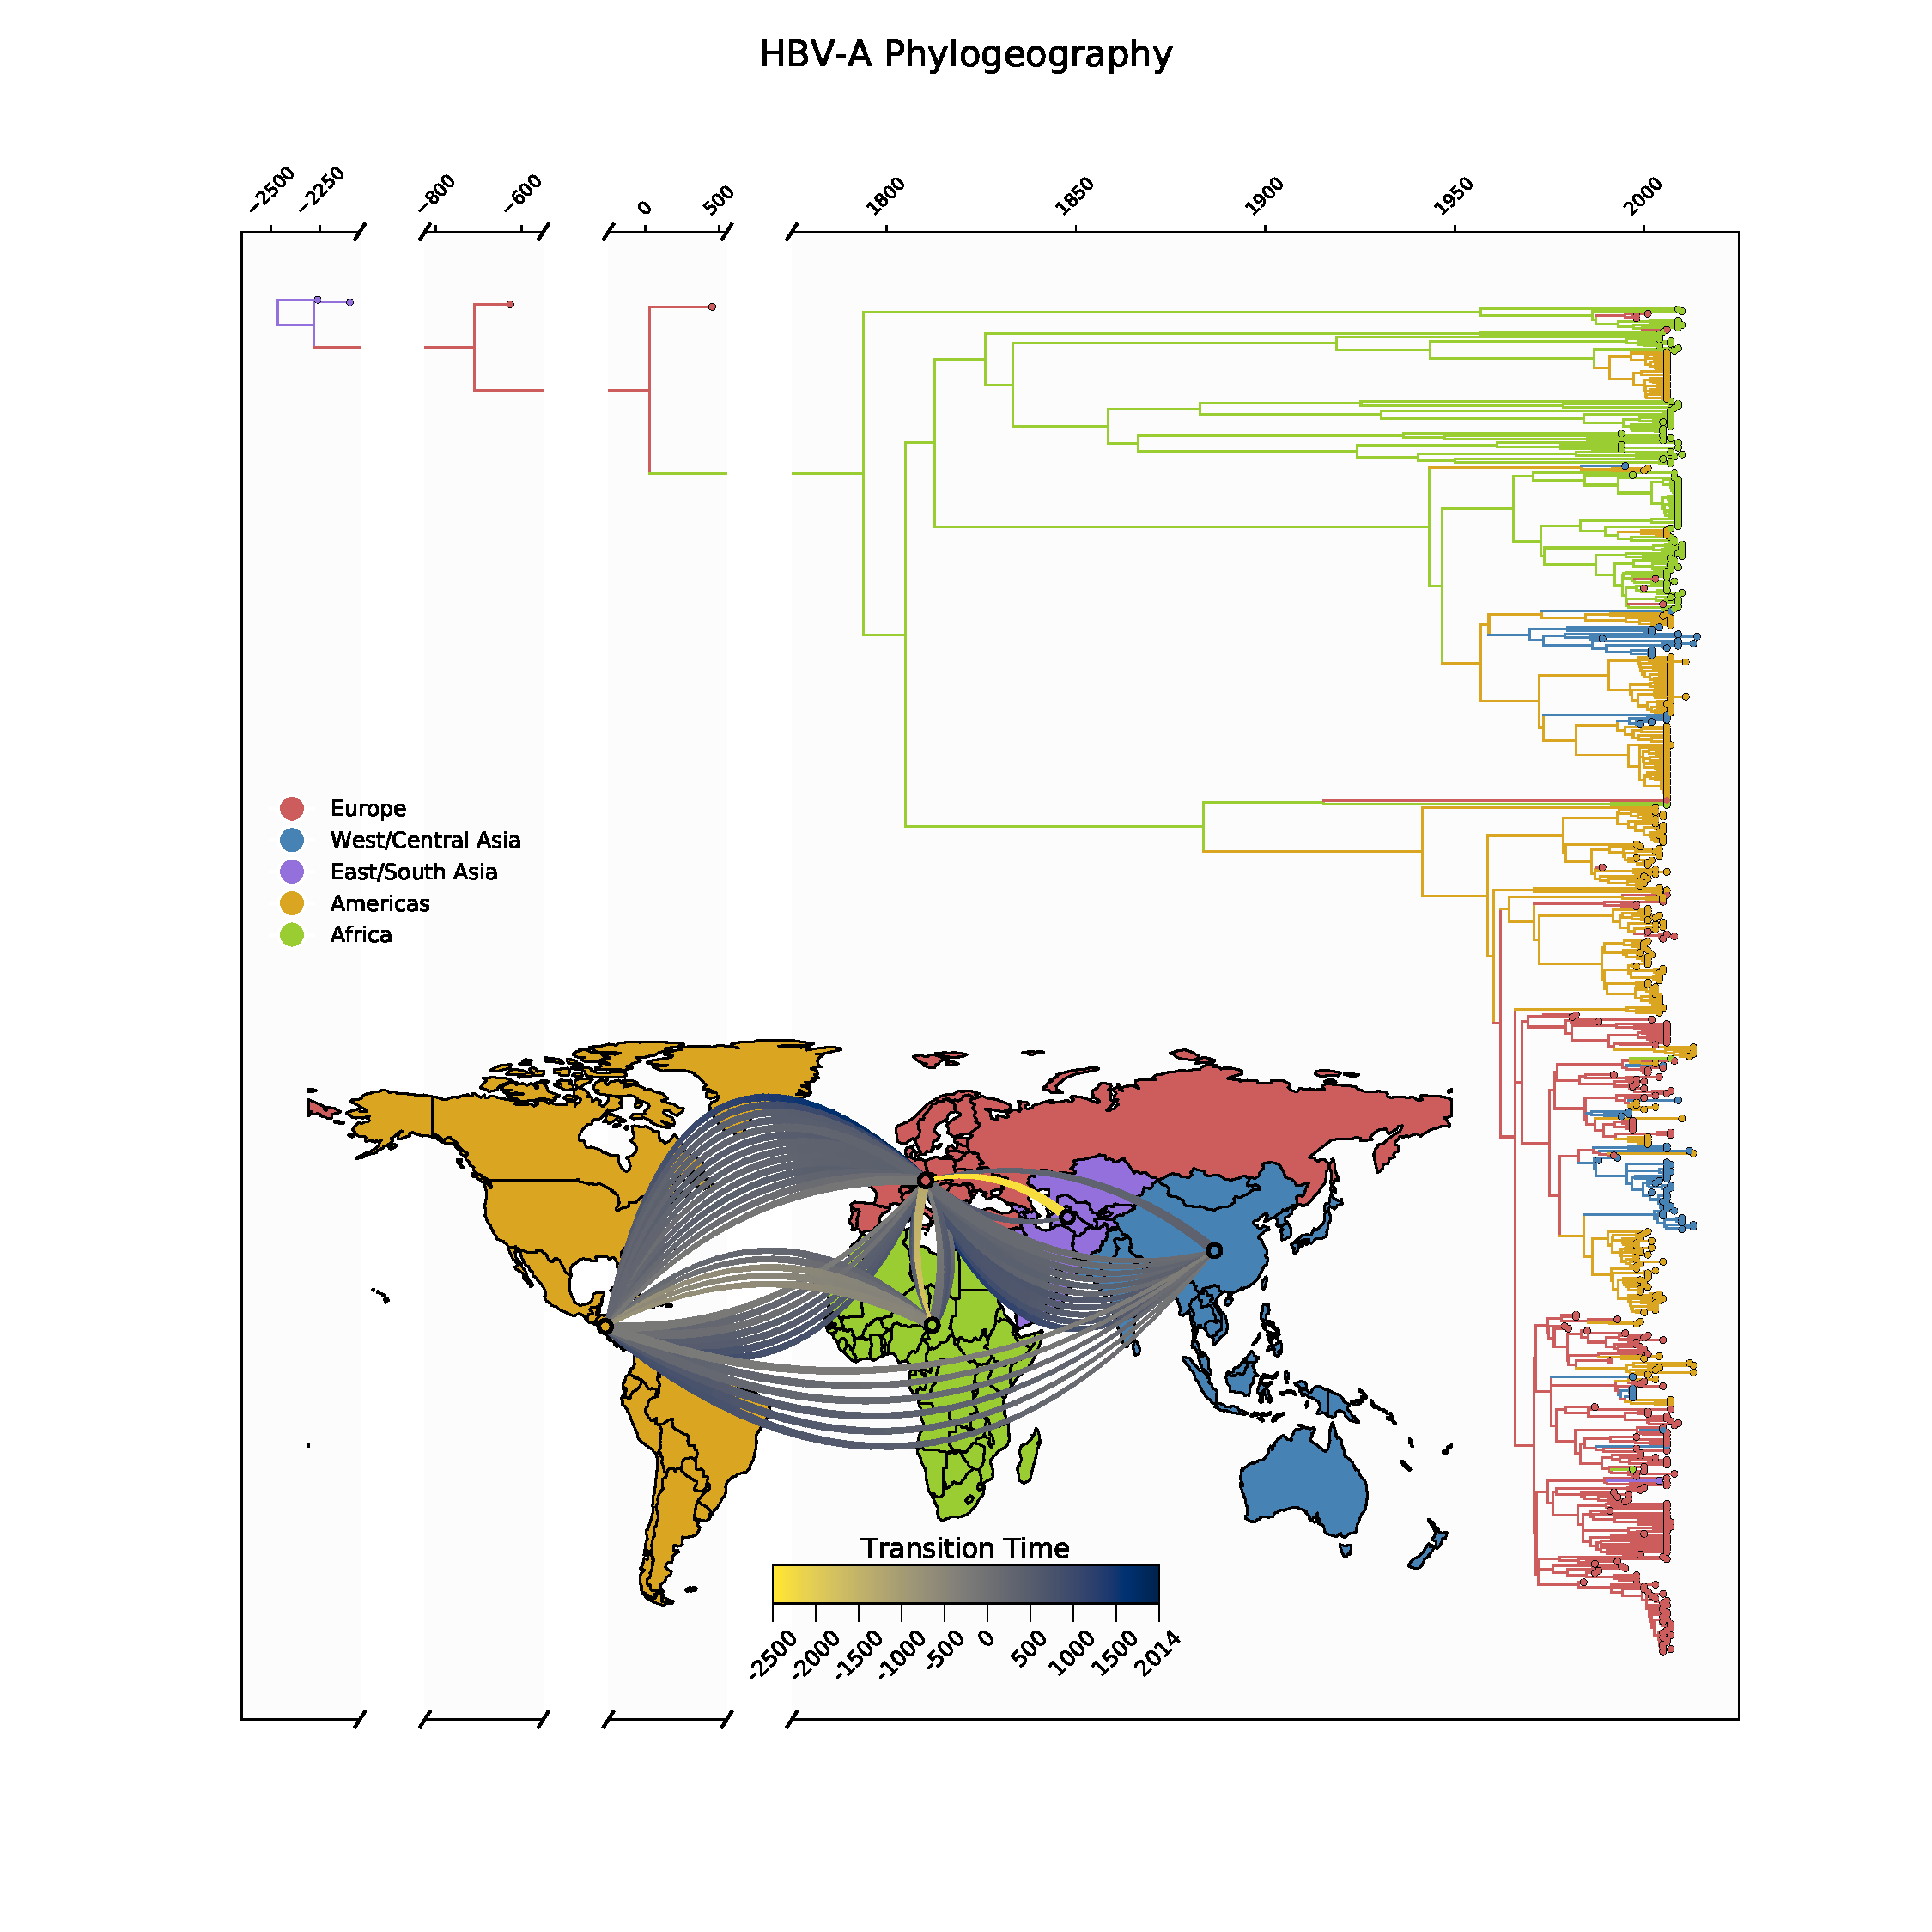
\includegraphics[width=\textwidth]{HBV-A_phylogeography_and_mcc_tree}
  \caption[HBV-A phylogeography ]{Time-scaled maximum clade credibility tree representing the evolutionary history of \gls{hbv} subtype A, averaged over 1,000 \gls{mcmc} posterior state samples. The root is inferred to be at 2504 BCE. Tip and branch colors represent location, both known and inferred by \gls{ctmc}. Breaks in time axis represent long periods of time covered by individual branches. (inset) World map colored according to regions used for \gls{ctmc} analysis. Each counterclockwise arrow represents an inferred transmission event between two regions (55 total). Arrow colors denote timing intervals of each introduction. Europe shows the greatest number of outgoing introductions (29). West \& Central Asia is the inferred root location of the tree, with one ancient transmission to Europe inferred to have taken place between 2243--876 BCE.}
  \label{fig:HBV-A_phylogeo}
\end{figure}

\begin{figure}[ht]
  \centering
  \medskip
  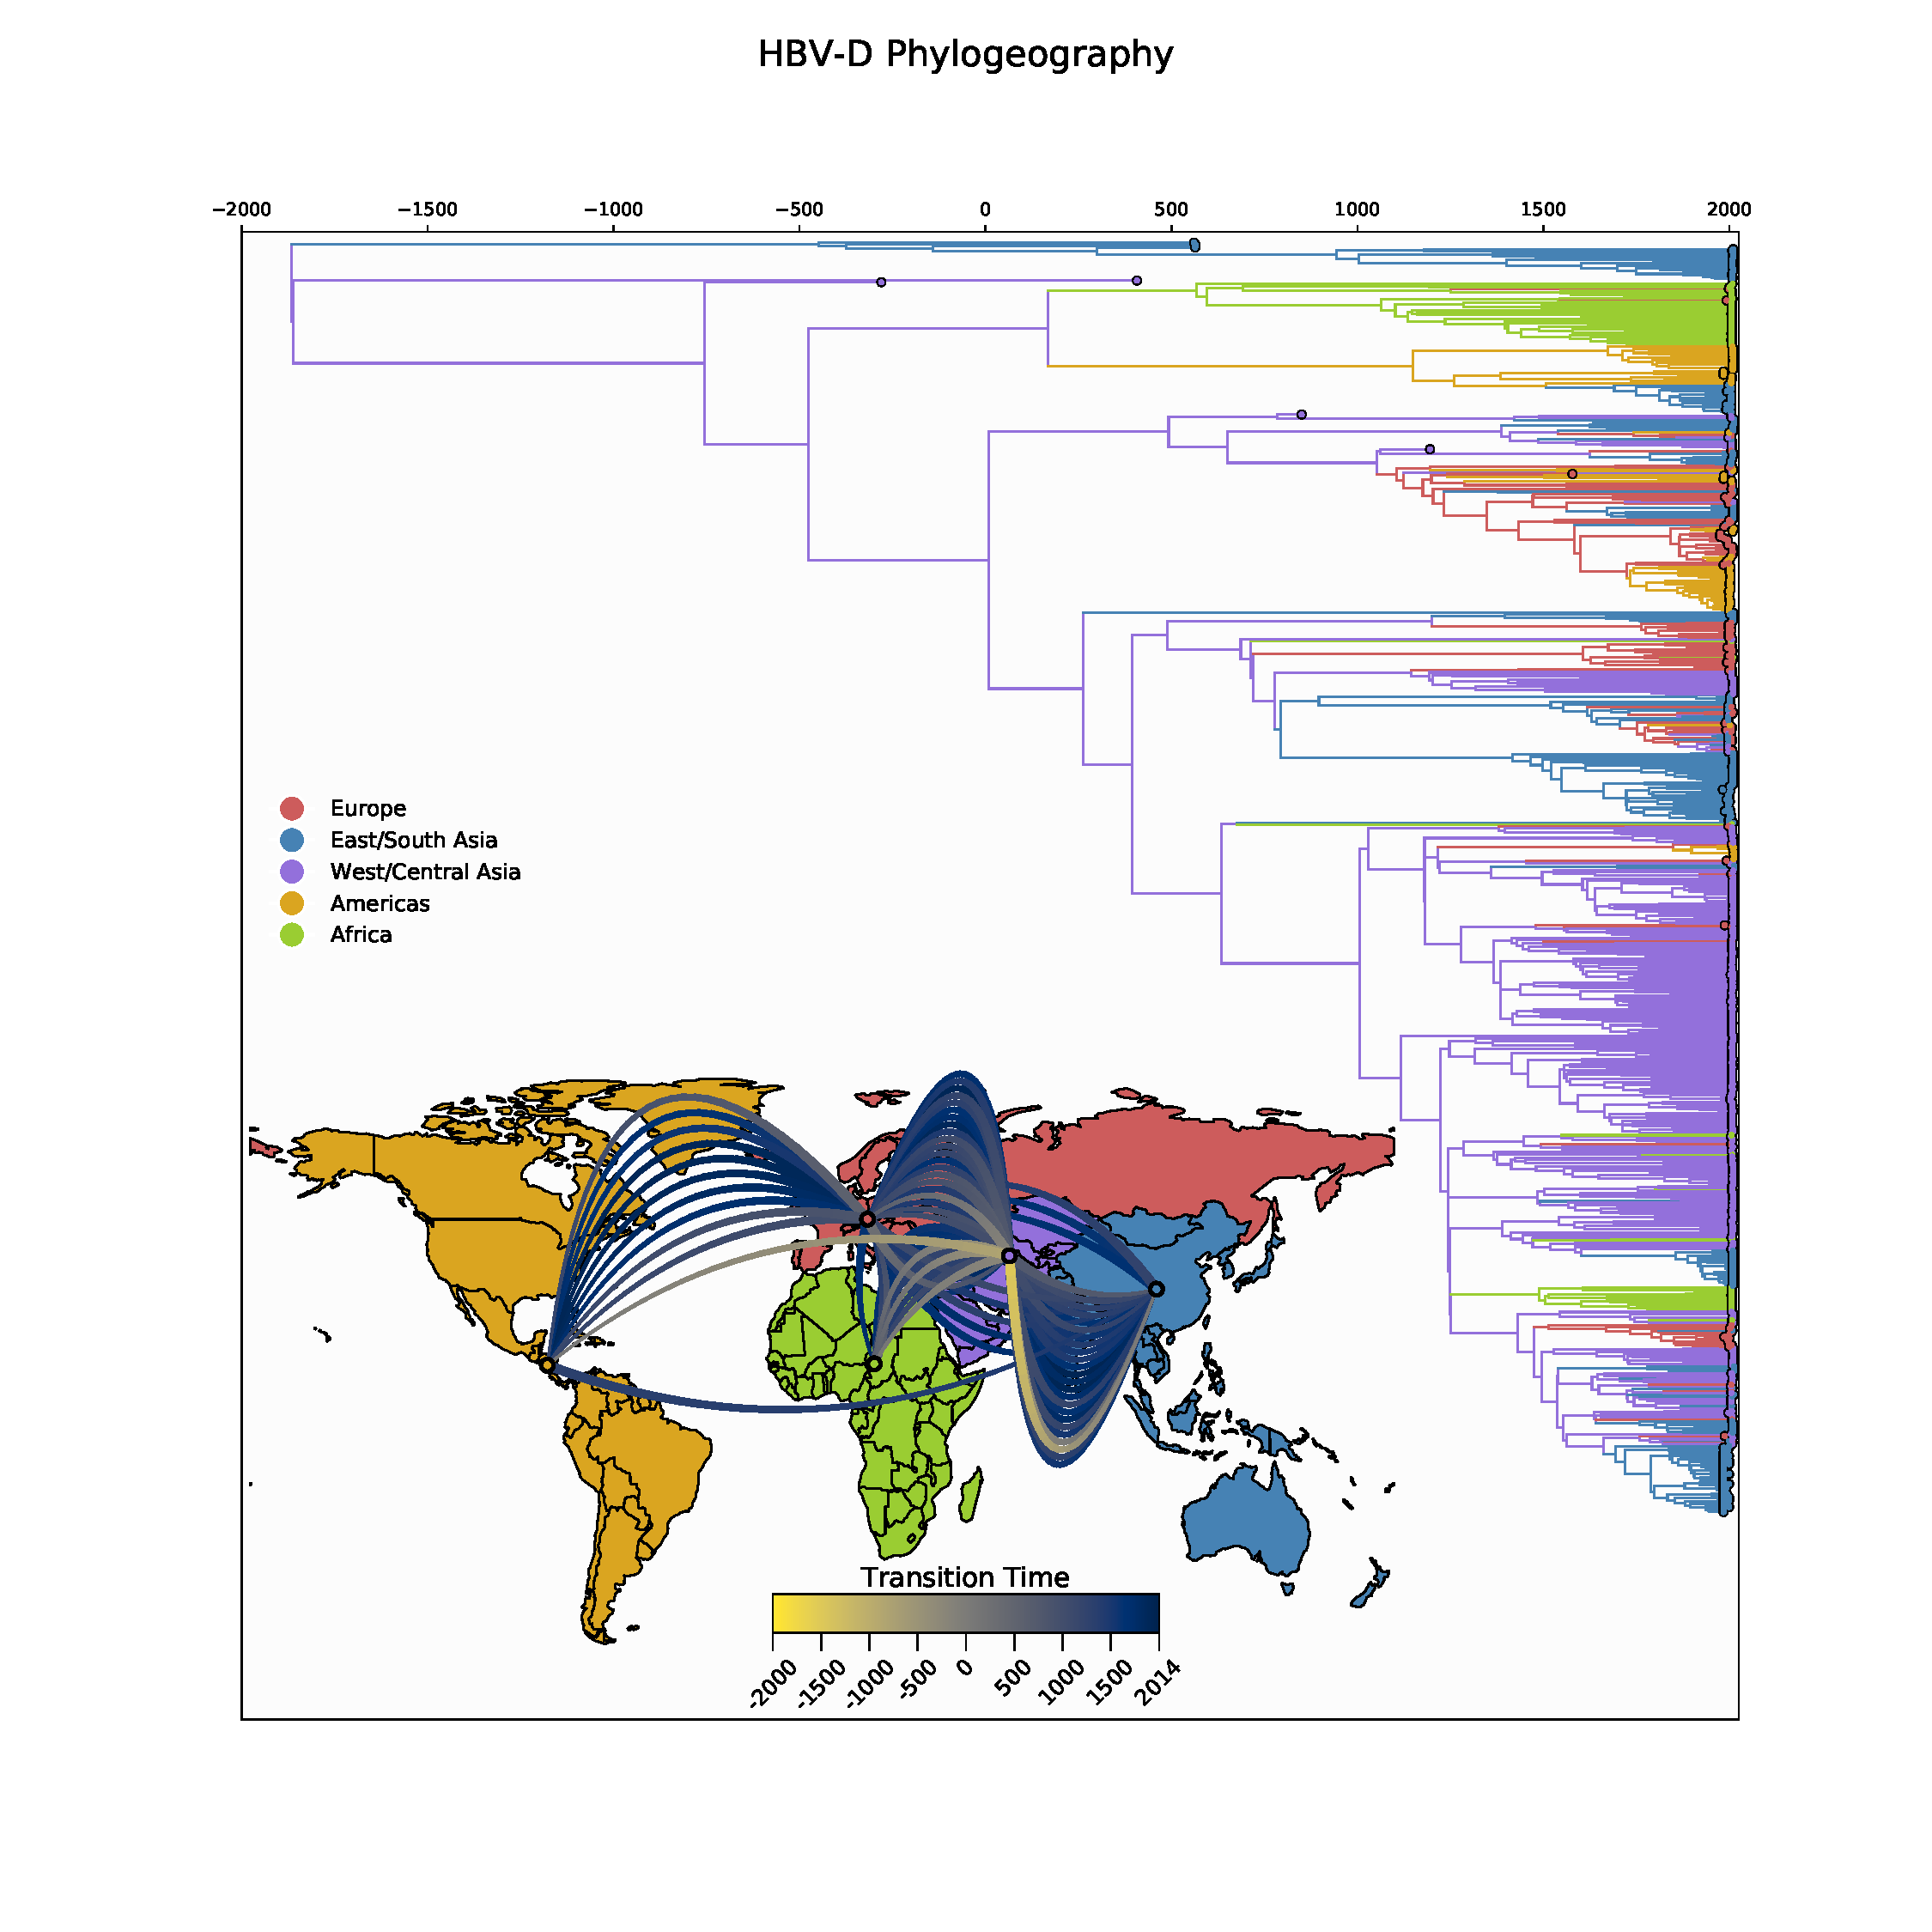
\includegraphics[width=\textwidth]{HBV-D_phylogeography_and_mcc_tree}
  \caption[HBV-D Phylogeography]{Time-scaled maximum clade credibility tree representing the evolutionary history of \gls{hbv} subtype D, averaged over 1,000 \gls{mcmc} posterior state samples. The root is inferred to be at 1779 BCE. Tip and branch colors represent location, both known and inferred by \gls{ctmc}. (inset) World map colored according to regions used for \gls{ctmc} analysis. Each counterclockwise arrow represents an inferred transmission event between two regions (82 total). Arrow colors denote timing intervals of each introduction. West \& Central Asia shows the greatest number of outgoing transmission events (55), as well as being the most likely location of the most recent common ancestor to sampled modern sequences.}
  \label{fig:HBV-D_phylogeo}
\end{figure}

\begin{figure}[ht]
  \centering
  \medskip
  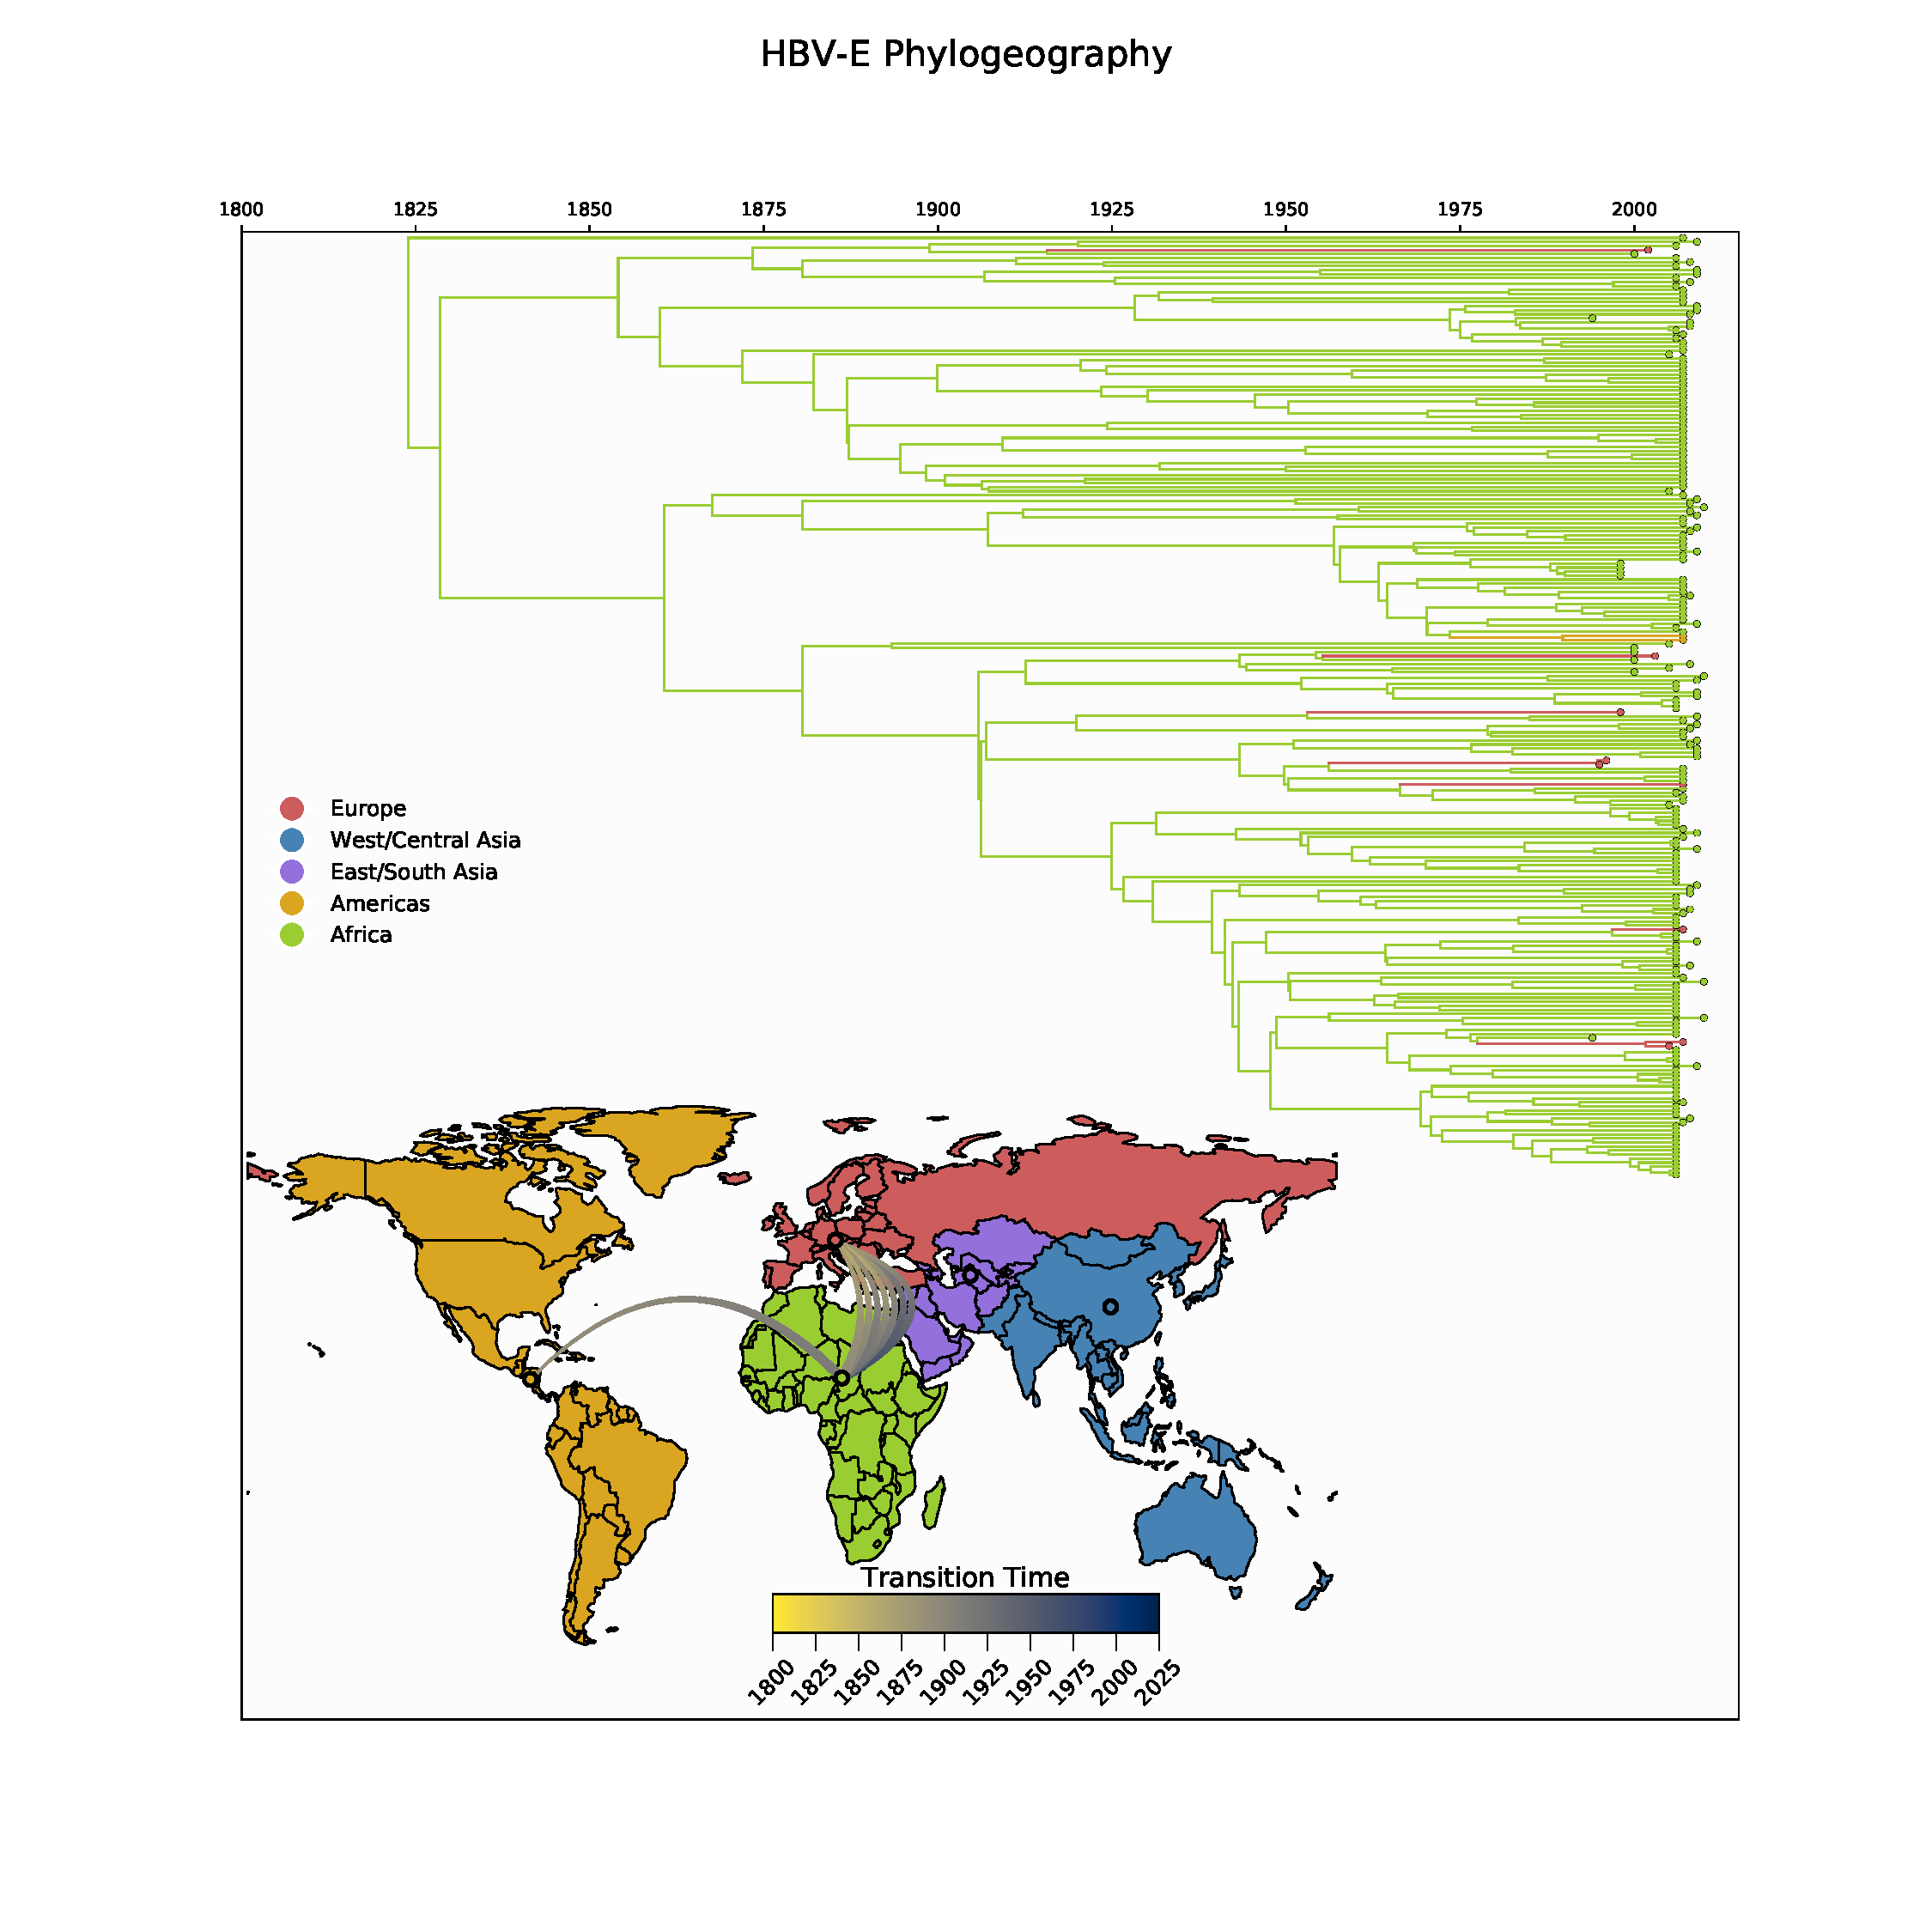
\includegraphics[width=\textwidth]{HBV-E_phylogeography_and_mcc_tree}
  \caption[HBV-E Phylogeography]{Time-scaled maximum clade credibility tree representing the evolutionary history of \gls{hbv} subtype E, averaged over 1,000 \gls{mcmc} posterior state samples. The root is inferred to be at 1824 CE. Tip and branch colors represent location, both known and inferred by \gls{ctmc}. Breaks in time axis represent long periods of time covered by individual branches. (inset) World map colored according to regions used for \gls{ctmc} analysis. Each counterclockwise arrow represents an inferred transmission event between two regions. Arrow colors denote timing intervals of each introduction. All migration events (8 total) are inferred to have originated in Africa; Europe was the destination of seven migrations, and the Americas were the destination of one.}
  \label{fig:HBV-E_phylogeo}
\end{figure}

\begin{figure}[ht]
  \centering
  \medskip
  \includegraphics[width=\textwidth]{bayes_factors}
  \caption[Bayes' factors of \gls{hbv} geographic transitions]{Networks summarizing posterior support for migrations between geographic regions as determined by \gls{bssvs} analysis. Inferred migrations are represented as counterclockwise arrows. Bayes' factors are represented by color intensity; darker arrows depict higher Bayes' factors, therefore higher posterior support. In \gls{hbv}-A we observe well supported inference of migrations out of Europe to all other regions, as well as high support for inferred migrations into Europe from Africa and the Americas. In \gls{hbv}-D we observe well supported migration history from Africa to Europe, and from Europe to the Americas and Asia. Finally, in \gls{hbv}-E we observe very well supported migration inference from Africa to Europe, as well as relatively high support for migration from Africa to the Americas.}
  \label{fig:bayes_factors}
\end{figure}

\section{Lassa phylogenetics}

For all Lassa analyses we present preliminary results which will motivate future work.
Using our adaptive workflow, we performed Bayesian phylogenetic inference on \gls{lasv} segments L and S under a Bayesian skygrid demographic model.
We ran \gls{mcmc} chains for segment L in parallel for a combined total of $1.5\times10^{12}$ states (excluding burn-in), and S for a combined total of $2.4\times10^{12}$ states (excluding burn-in).
We note that this analysis took almost a month of computational time on the Vlaams Supercomputer Centrum cluster, parallelized across three independent replicates per segment.
This represents a total computational time of roughly 6 months.

Our inference revealed markedly different clock rates between the two segments.
In segment L we infer a mean clock rate of $9.9914\times10^{-4}$ substitutions per site per year [95\% HPD:$9.0332\times10^{-4}$--$1.0646\times10^{-3}$].
In segment S we instead infer a mean clock rate of $2.2116\times10^{-3}$ substitutions per site per year [95\% HPD:$1.9757\times10^{-3}$--$2.4948\times10^{-3}$].
While this estimate for the clock rate of segment L is concordant with rates established for \gls{lasv} in the literature\cite{andersen2015clinical, fichet2016spatial}, our estimate for segment S differs from the literature by a factor of 10 (Fig.~\ref{fig:lassa_clock_rates}).
Despite this difference, we find overlapping estimates of \gls{tmrca} for the two segments: 1698 CE for segment L and 1752 for segment S.
Additionally, we performed Bayesian skygrid reconstruction of the demographic history of both segment L (Fig.~\ref{fig:l_skygrid}) and segment S (Fig.~\ref{fig:s_skygrid}).
Both segments' population reconstructions show the same patterns.
In both segments we observe exponentially increasing effective population size since the \gls{tmrca} until roughly 1900.
The 1900s show a trough in effective population size (lowest around the year 1950) followed by another increase in population until roughly the 1990s.
Over the last three decades, we observe much more variable growth and decline in population size, with sharp dips in inferred population size in the late 1990s and since the year 2015.

\begin{figure}[ht]
  \centering
  \medskip
  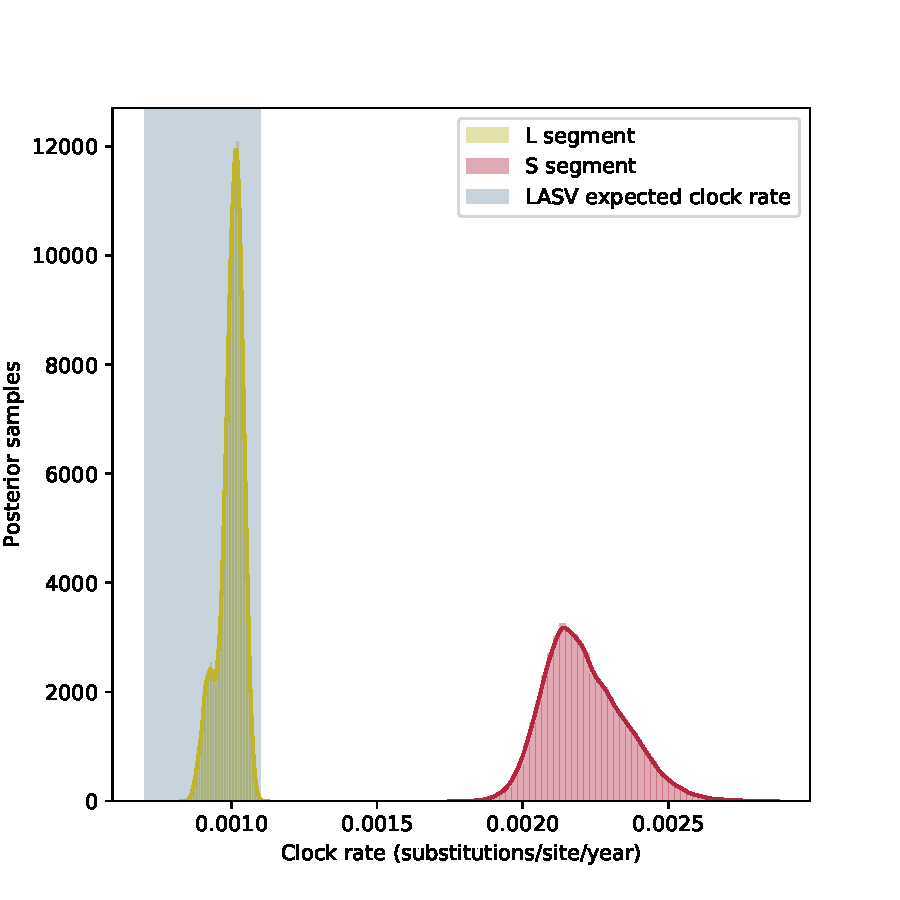
\includegraphics[width=.9\textwidth]{clock_rates_by_segment}
  \caption[LASV clock rates by segment]{Histograms and kernel density estimates of mean clock rate posterior samples in \gls{lasv} segments L (green) and S (red). Blue shaded region represents expected clock rate range (7--11)$\times10^{-4}$ substitutions per site per year), as derived from the literature on Lassa virus clock rates\cite{andersen2015clinical, fichet2016spatial}. While segment L's clock rate falls within the expected window, segment S demonstrates a clock rate roughly tenfold higher than expected.}
  \label{fig:lassa_clock_rates}
\end{figure}

\begin{figure}[ht]
  \centering
  \medskip
  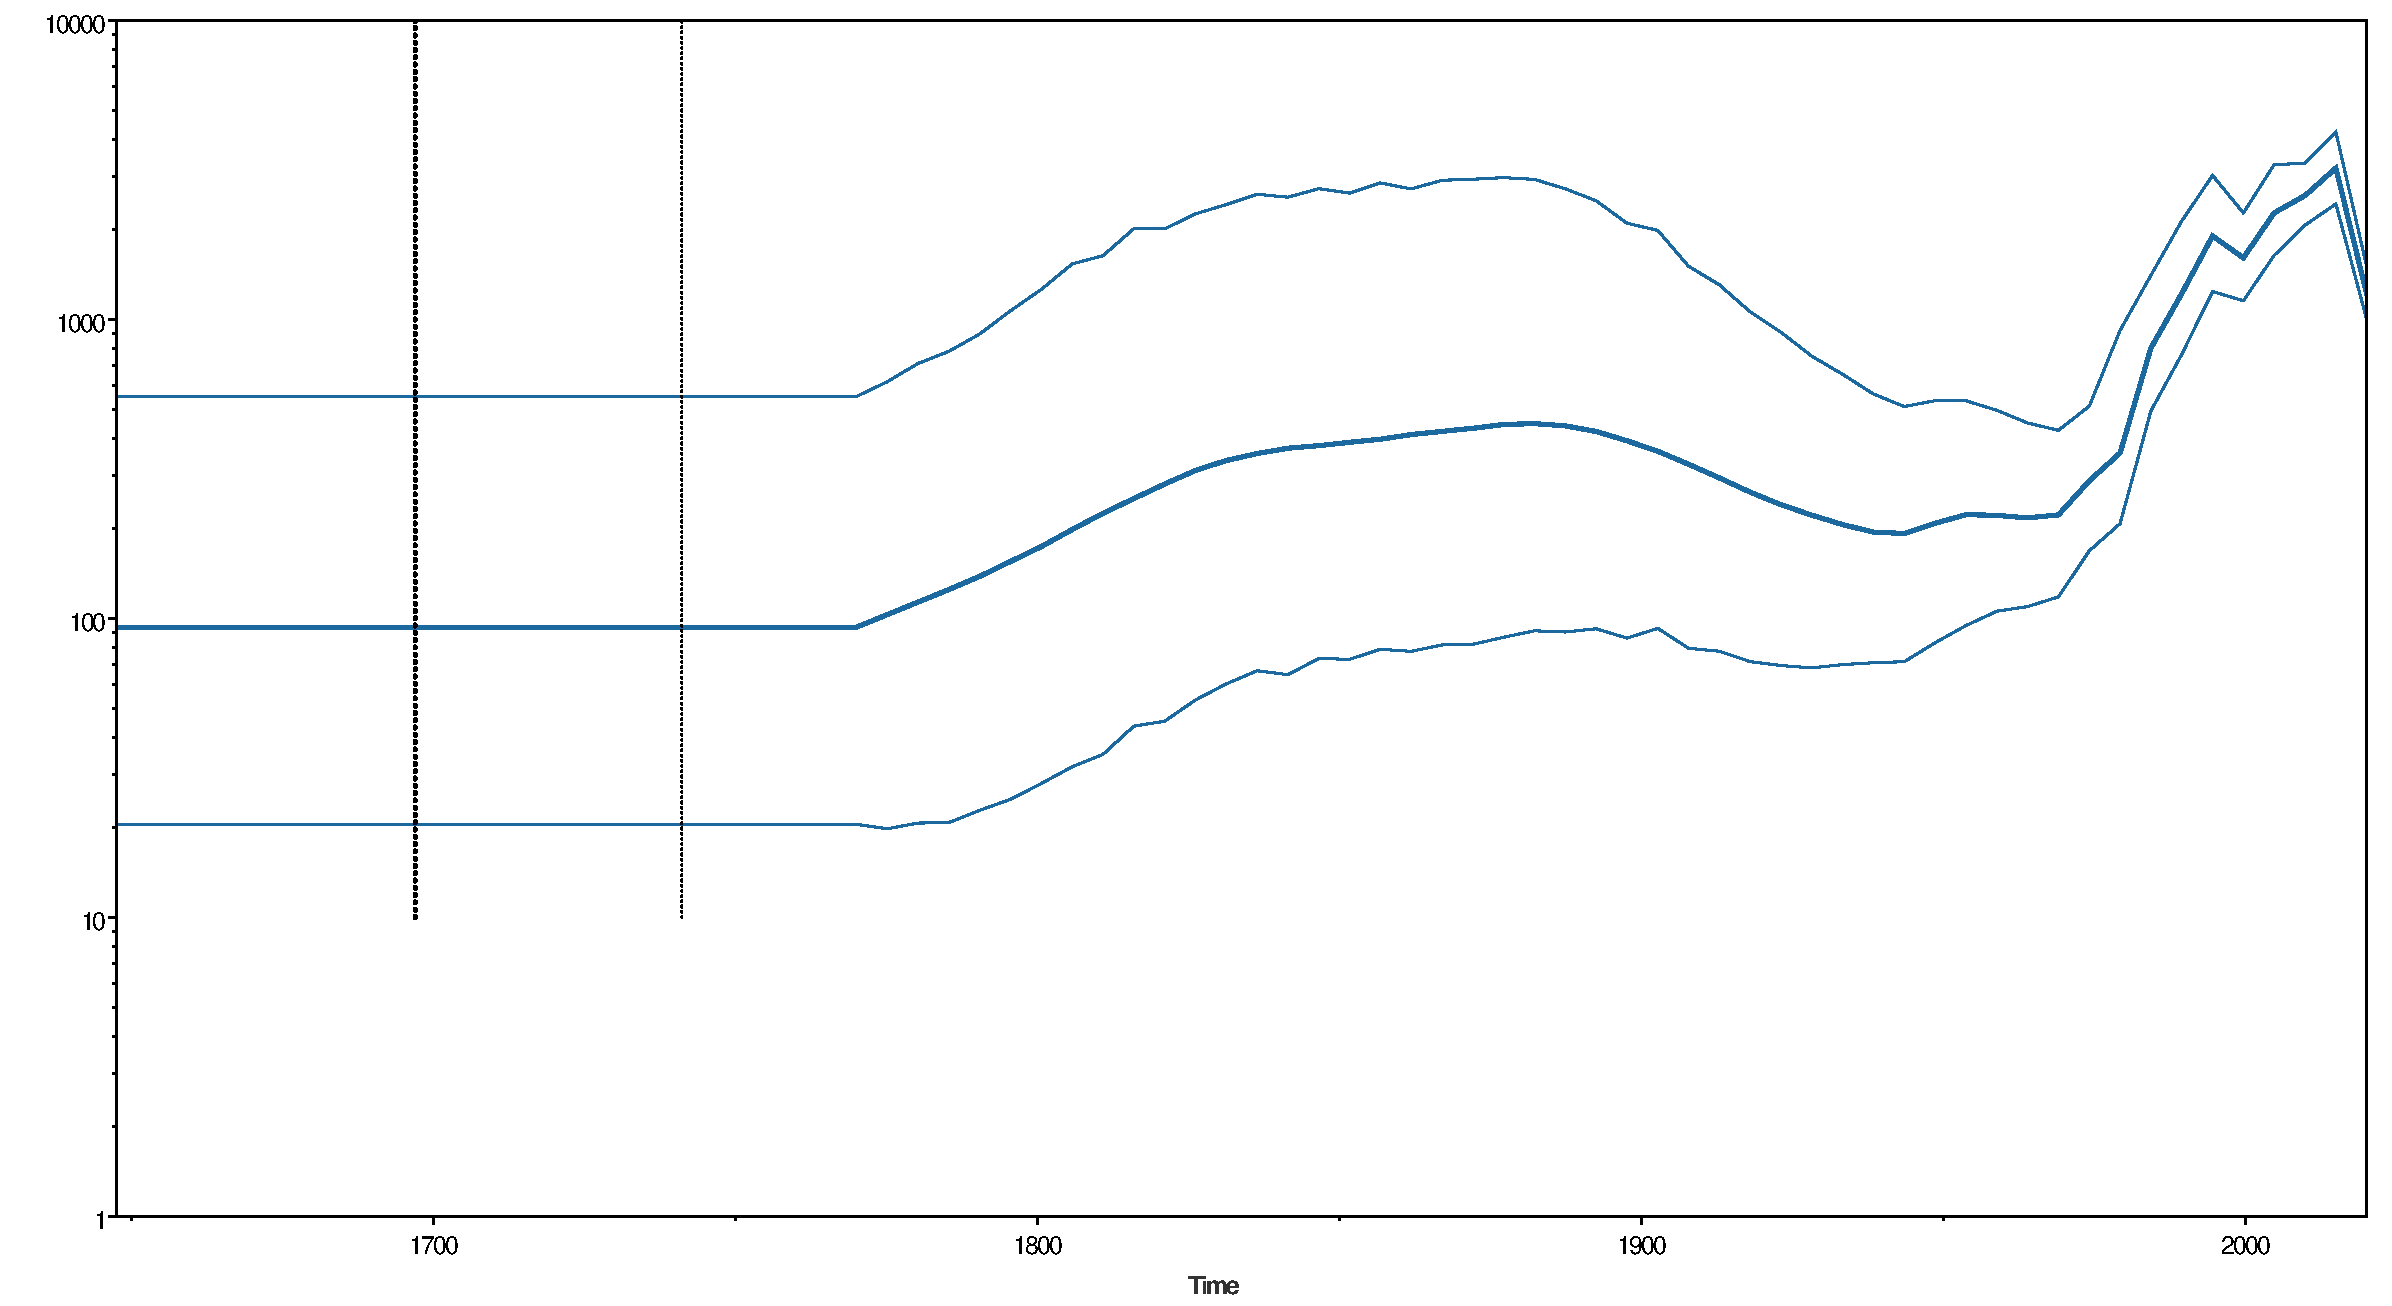
\includegraphics[width=.9\textwidth]{l_skygrid_population_reconstruction}
  \caption[Demographic history of Lassa's L segment]{Bayesian skygrid reconstruction of the demographic history (effective population size over time) of \gls{lasv} segment L. Dashed vertical lines denote the mean root age and 95\% HPD interval: 1697 [1647--1741].}
  \label{fig:l_skygrid}
\end{figure}

\begin{figure}[ht]
  \centering
  \medskip
  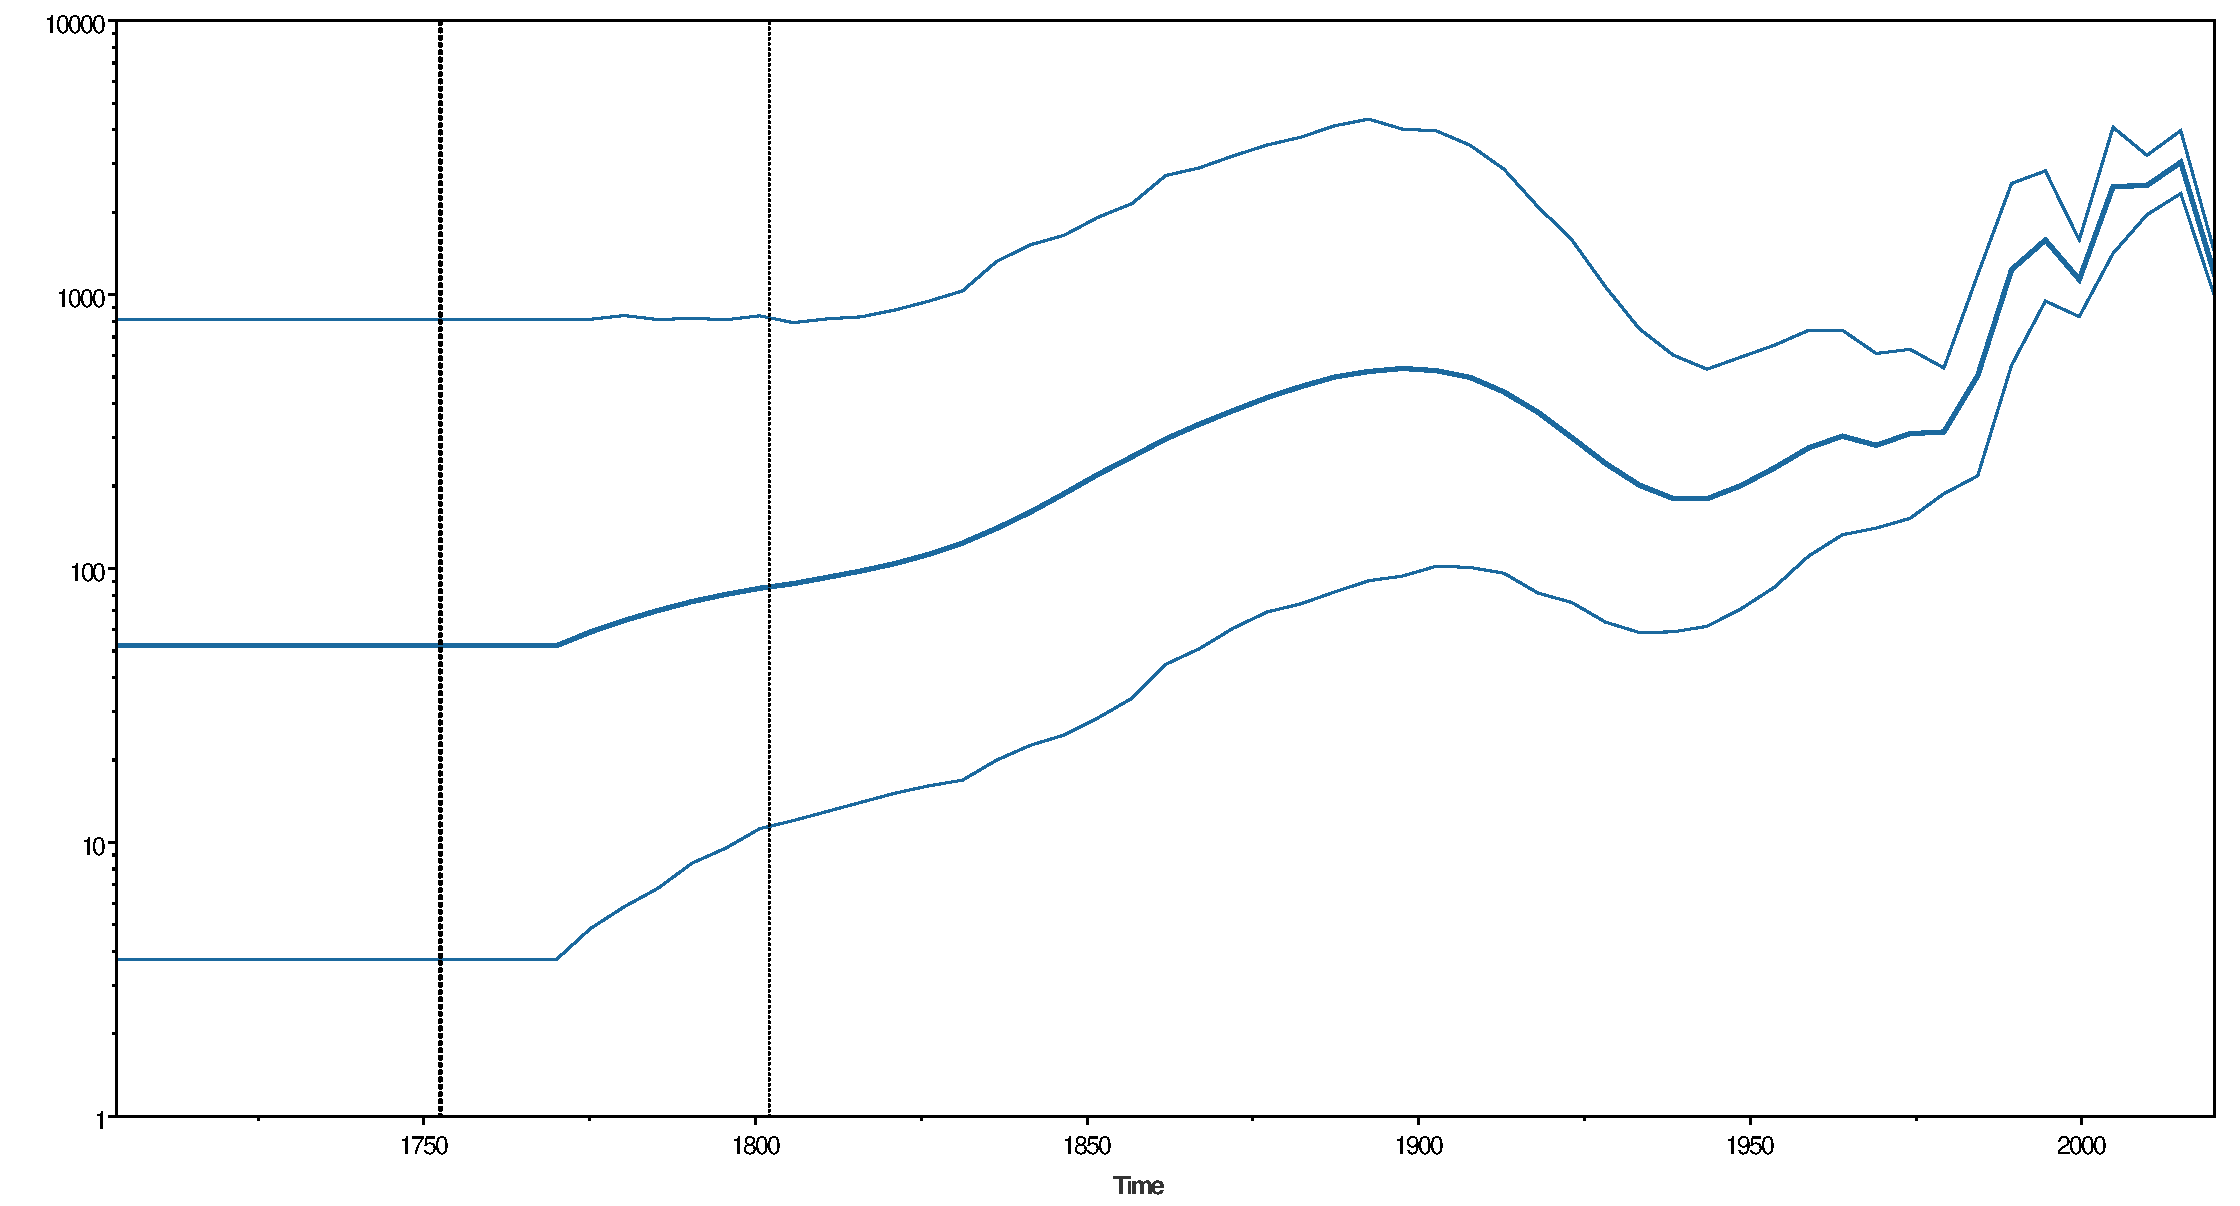
\includegraphics[width=.9\textwidth]{s_skygrid_population_reconstruction}
  \caption[Demographic history of Lassa's S segment]{Bayesian skygrid reconstruction of the demographic history (effective population size over time) of \gls{lasv} segment S. Dashed vertical lines denote the mean root age and 95\% HPD interval: 1752 [1751--1802].}
  \label{fig:s_skygrid}
\end{figure}


%%%%%%%%%%%%%%%%%%%%%%%%%%%%%%%%%%%%%%%%%%%%%%%%%%
% Keep the following \cleardoublepage at the end of this file,
% otherwise \includeonly includes empty pages.
\cleardoublepage

% vim: tw=70 nocindent expandtab foldmethod=marker foldmarker={{{}{,}{}}}
